\documentclass{article}
\usepackage[ngerman]{babel}
\usepackage{graphicx}
\usepackage{xcolor}
\usepackage{shapepar}
\usepackage{scrpage2}
\pagestyle{scrheadings}
\clearscrheadfoot
\ohead{\pagemark}
\ihead{Eine Buchrezension von Evelyn Ortler}
\ifoot{\today}

\begin{document}
\maketitle
\begin{center}
\subtitle{\bfseries \Huge Der Schein der Weisen} \newline
\title{\Large Irrt\"{u}mer und Fehlurteile im t\"{a}glichen Denken}\newline  

\end{center}

\begin{figure}[htbp]
	\centering
		
\includegraphics{Cover.jpg}
	\label{fig:Cover}
\end{figure}
\newpage



\begin{center}
\subparagraph{\LARGE Aufbau des Buches}
\newline
\newline
\paragraph{Das Buch ist in vier Teile eingeteilt:}
\begin{itemize}
	\item Teil 1: Der Anfang vom Ende
	\item Teil 2: Kein Urteil ohne Vor-Urteil
	\item Teil 3: Die Lebensl\"{u}ge der medizinischen Forschung
	\item Teil 4: Am Ende ein neuer Anfang
\end{itemize}
\end{center}


\begin{text}
\large
Jeder dieser Teile ist wiederum in Kapitel unterteilt. \newline
Die \"{U}berschriften sind sehr gut gew\"{a}hlt!! \newline
Auch sind in diesem Buch zahlreiche Tabellen abgebildet, eine davon ist hier \"{u}bernommen:
\end{flushleft}
\end{text}

\begin{tabbing}
\=Fisch n\"{a}hert sich dem Spezialk\"{o}der auf einen Meter& \=Fisch bei{\ss}t an  &\=Fisch bei{\ss}t nicht an\\
\>Leckerellen																								&	\=100\%								&\=  0\% \\
\>Ekelitzen																									&	\=	5\%								&	\= 95\% \\


\end{tabbing}

\captionbelow{Ein Beispiel vom Angeln der Leckerellen und Ekelitzen}
\newline

\begin{figure}[htbp]
	\centering
		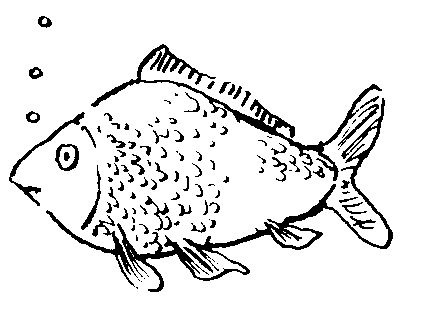
\includegraphics{fisch.jpg}
	\label{fig:fisch}
\end{figure}

\newline
\newpage




\begin{flushleft}
		\subtitle \textcolor{blue}{\scshape Einige Kostproben der Spr\"{u}che und Zitate aus dem Buch\\
		Alle guten Dinge sind DREI =)}
\end{flushleft}
		
		\begin{verse}	
		\fbox{{Aus dem Kapitel: Gru\ss} ins Blaue}}\newline
		\newline
		Eine Katze hat einen Schwanz mehr als keine Katze.\newline
		Keine Katze hat sieben Schw\"{a}nze.\newline
		Also hat eine Katze acht Schw\"{a}nze.\newline
		\end{verse}
		\newline
		\newline
		
		\begin{verse}
		\fbox{Aus dem Kapitel: Wo bleibt Hartmut?}\newline
		\newline
		\newline
		Wer Eier nach Gef\"{u}hl kocht,\newline
		wird mit Wahrscheinlichkeiten auch nicht anders umgehen.\newline
		\small{\itshape Hans-Hermann Dubben}
		\end{verse}
		\newline
		\newline
		
		\begin{verse}
		\fbox{Aus dem Kapitel: Was dich umbringt, bringt mich voran}\newline
		\newline
		\newline
		Man kann alle Leute einige Zeit zum Narren halten\newline
		und einige Leute allezeit;\newline
		aber alle Leute allezeit zum Narren halten kann man nicht.\newline
		\small{\itshape Abraham Lincoln}
		\end{verse}
\newpage

\subparagraph {\large Minimale Information zu den Autoren}\newline
\newline
\begin{flushleft} \newline 
Prof. Dr. Hans-Peter Beck-Bornholdt und Privatdozent Dr. Hans-Hermann Dubben wurden bekannt durch ihr vergn\"{u}gliches Buch "Der Hund, der Eier legt". Beide lehren an der Universit\"{a}t in Hamburg Medizin. Von Haus aus sind sie jedoch Physiker. Sie haben verschiedene akademische Preise erhalten, unter anderem den Fischer-Appelt-Preis der Universit\"{a}t Hamburg im Jahr 1996 f\"{u}r hervorragende Leistungen.
\end{flushleft}
\begin{figure*}[h]
	\centering
		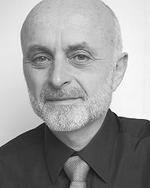
\includegraphics{dubben.jpg}
	\caption{Hans-Hermann Dubben}
	\label{fig:dubben}
\end{figure*}
\begin{figure*}[h]
	\centering
		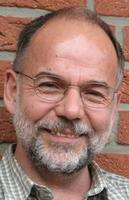
\includegraphics{bebo.jpg}
		\caption{Hans-Peter Beck-Bornholdt}
	\label{fig:bebo}
\end{figure*}
\newpage


	\subparagraph {\Huge Inhaltsangabe \newline
	\small Zusammenfassung des ersten gro{\ss}en Teiles des Buches}
	\begin{flushleft}
	\begin{text}	\newline
	Marina f\"{a}hrt einen blauen Golf. Wenn wir einen blauen Golf vorbei fahren sehen und daraus schlie{\ss}en, dass 			Marina am Steuer sitzt, obwohl das nicht zutrifft, begehen wir einen Fehler erster Art.\newline
	Wenn wir keinen blauen Golf sehen, glauben wir auch keine Marina zu sehen, dabei f\"{a}hrt sie gerade mit einem 				wei{\ss}en Leihwagen vorbei. Wir begehen einen Fehler zweiter Art.\newline
	Das Gru{\ss}verhalten.\newline
	In der Innenstadt gibt es viele blaue Golfs, in denen keine Marina sitzt, damit ist der Fehler erster Art fast schon 		vorprogrammiert, d.h. wir gr\"{u}{\ss}en nicht. \newline
	In der Sackgasse, in der Marina wohnt soll man blaue Golfs jedoch immer gr\"{u}{\ss}en, denn es ist sehr 								wahrscheinlich, dass Marina am Steuer sitzt. \newline
	Andreas f\"{a}hrt ein Feuerwehrauto, er nennt es Paulchen, es hat ganz besondere Kennzeichen. Wenn Paulchen 						vorbeif\"{a}hrt sitzt immer Andreas am Steuer, egal wo man ist. \newline
	\newline
In manchen Situationen aber reicht es einfach nicht, nur H\"{a}ufigkeitsrechnungen anwenden zu k\"{o}nnen! So zum Beispiel beim Fischen. \newline
Thoma's Anglergl\"{u}ck h\"{a}ngt nicht nur vom Spezialk\"{o}der ab, den er verwendet, sondern auch vom Vorkommen der Leckerellen und Ekelitzen im Wasser. \newline
Auch wenn Marina und Celina zu Hause auf ihre M\"{a}nner warten und beide nicht kommen, k\"{o}nnen sie sich \"{u}ber die Vorinformationen Gedanken machen. Beispielsweise kommt Celinas Mann niemals zu sp\"{a}t, das hei{\ss}t, es ist sehr wahrscheinlich, dass ihm etwas zugesto{\ss}en ist. Marinas Mann hingegen ist sehr unp\"{u}nktlich, daraus kann man schlie{\ss}en, dass es Mario wahrscheinlich gut geht.\newline
Die Einsch\"{a}tzung eines Ereignisses h\"{a}ngt nicht nur von den unmittelbaren Fakten ab, sondern auch von den Vorinformationen, die man hat. Verschiedene Personen kommen aber zu unterschiedlichen Schlussfolgerungen, da sie unterschiedliche Erfahrungen haben und somit verschieden an das Ereignis herangehen.
\end{text}
\end{flushleft}
\newpage


\heartpar{\Large Meine Meinung zum Buch \normalsize Anfangs nach den ungef\"{a}hr ersten zwei Kapiteln hab ich mir gedacht \glqq Mein Gott! Was hab ich mir denn gerade dieses Buch ausgesucht! \grqq Aber nach dem ersten Teil des Buches hat es mir dann schon besser gefallen. Und als ich dann merkte, dass die Autoren des Buches eigentlich manchmal ganz witzige Ausschnitte einbringen war ich dann fast schon begeistert vom Buch. Gefehlt hat mir ein wenig, dass nicht ein einziges Mal erw\"{a}hnt wurde, wie nun diese Wahrscheinlichkeitsrechnung eigentlich ausschaut. Sonst im gro{\ss}en und ganzen hat es mir imponiert.=) Auch nett sind die zahlreichen, gro{\ss}teils lustigen, Karikaturen im Buch. Die Tabellen hingegen wurden mir manchmal zu viel! Aber das Buch ist auf alle F\"{a}lle allen Mathematikbegeisterten d.h. sowieso allen Wisslyzern zu empfehlen! =P! \heartsuit}
\newpage



\begin{text}
\begin{flushleft} \newline
Das ganze Buch basiert ja eigentlich auf dem \newline \begin{center} \LARGE Bayes'schem Theorem \end{center} \newline \normalsize und deshalb ist es hier zum Schluss noch angef\"{u}hrt:

\large Thomas Bayes war ein englischer Pfarrer und Mathematiker.\newline
Bayes hat den Ansatz f\"{u}r die Wahrscheinlichkeitsrechnung gefunden.\newline
Oft geht es n\"{a}mlich darum die wahrscheinlichste Hypothese aus vielen Hypothesen herauszusuchen.\newline
Durch das Bayes'sche Theorem wird das m\"{o}glich.
\newline
\newline
Zum Schluss meiner Buchrezension noch das allgemeine Bayes'sche Theorem:
\newline
$p(m+|v+) = \frac{p(m+)* p(v+|m+)}{p(m+)*p(v+|m+) + p(m-)*p(v+|m-)}$
\end{flushleft}
\end{text}


\end{document}